%% Chapter 1
\chapter{Introduction} % Main chapter title
%\label{sens_introduction} % For referencing the chapter elsewhere, use \ref{sens_introduction} 
%%%%%%%%%%%%%%%%%%%%%%%%%%%%%%%%%%%%%%%%%%%%%%%%%%
%%%%%%%%%%%                                                     %%%%%%%%%%%%%%%%%%%%%%%%%%%
%%%%%%%%%%%           1.1   Depth Camera Application                   %%%%%%%%%%%%%%%%%%%%
%%%%%%%%%%%                                                     %%%%%%%%%%%%%%%%%%%%%%%%
%%%%%%%%%%%%%%%%%%%%%%%%%%%%%%%%%%%%%%%%%%%%%%%%%%%
%\section{Depth Camera Application}
%
%As the depth camera technology opens a new epoch for three-dimensional (3D) markets, the multimedia technologies development is changing from two-dimensional (2D) to 3D on games, movies, health care aid, military training, etc., all various areas that are in demand of a more direct reflection on the real world \cite{depthOverview12}. Simple 2D scenes are not able to meet the social demands any more. And with the fast development of multimedia technologies, three-dimensional (3D) scene display has become a hotspot in the display field. As an extension of classic 2D video, the 3D dynamic display technology can provide a more comprehensive immersive feeling to users than a 2D video. Gesture recognition, 3D modeling, 3D printing, augmented reality, virtual reality, etc., a lot of ongoing researches and applications on depth cameras are famous now, cooperated with Human Computer Interaction (HCI) technologies.
%\\\\%
%Pattern recognition and gesture recognition are of the hottest sustained research activities in the area of HCI. Being a significant part in non verbal communication hand gestures are playing vital role in our daily life. Hand Gesture recognition system provides us an innovative, natural, user friendly way of interaction with the computer which is more familiar to the human beings. Gesture Recognition has a wide area of application including human machine interaction, sign language, immersive game technology etc. By keeping in mind the similarities of human hand shape with four fingers and one thumb, \cite{gestureRecognition12} present a real time system for hand gesture recognition on the basis of detection of some meaningful shape based features like orientation, center of mass (centroid), status of fingers, thumb in terms of raised or folded fingers of hand and their respective location in image.
%\\%
%Since gestures based on hand and finger movements can be robustly understood by computers by using a special 3D IR camera, users are allowed to play games and interact with computer applications in natural and immersive ways that improve the user experience. In 2010, Microsoft's first generation Kinect, using PrimeSense’s technology, is based on projecting a structured light pattern on the object in order to build and track the skeleton of the user’s body to control a series of electronic games. \cite{SL3Dfrom2D96} also discussed similar techniques for 3D object reconstruction. By using this depth-map along with the 2D color images obtained via the Kinect camera, the computational unit of the Xbox 360 console was capable of providing a fairly robust gesture recognition solution. After \cite{KinectGesture12} proposed two methods for gesture recognition, a plethora of applications have been produced around Kinect by various groups of image processing researchers.
%\\%
%A Kinect-based calling gesture recognition scenario is proposed by \cite{gestureKinect14} for taking order service of an elderly care robot. Its proposed scenarios are designed mainly for helping non expert users like elderly to call service robot for their service request. In order to facilitate elderly service, natural calling gestures are designed to interact with the robot. Individual people is segmented out from 3D point cloud acquired by Microsoft Kinect, skeleton is generated for each segment, face detection is applied to identify whether the segment is human or not, specific natural calling gestures are designed based on skeleton joints. \cite{NIRGesture14} proposed another smart and real-time depth camera based on a new depth generation principle. A monotonic increasing and decreasing function is used to control the frequency and duty-cycle of the NIR illumination pulses. The adjusted light pulses reflect off of the object of interest and are captured as a series of images. A reconfigurable hardware architecture calculates the depth-map of the visible face of the object in real-time from a number of images. The final depth map is then used for gesture detection, tracking and recognition.
%\\\\%
%3D printing is an additive technology in which 3D objects are created using layering techniques of different materials, such as plastic, metal, etc.  It has been around for decades, but only recently is available and famous among the general public. The first 3D printing technology developed in the 1980’s was stereolithography (SLA) \cite{Patent3Dprinting86}. This technique uses an ultraviolet (UV) curable polymer resin and an UV laser to build each layer one by one. Since then other 3D printing technologies have been introduced.
%%
%Nowadays, some companies like iMaterialise or Shapeways offer 3D printing services where you can simply upload your CAD model on-line, choose a material and in a few weeks your 3D printed object will be delivered to your address. This procedure is quite straight-forward when you got your CAD model. However, 3D shape design tends to be a long and tedious process, with the design of a detailed 3D part usually requiring multiple revisions. Fabricating physical prototypes using low cost 3D fabrication technologies at intermediate stages of the design process is now a common practice, which helps the designer discover errors, and to incrementally refine the design. Most often, implementing the required changes directly in the computer model, within the 3D modeling software, is more difficult and time consuming than modifying the physical model directly using hand cutting, caving and sculpting tools, power tools, or machine tools. When one of the two models is modified, the changes need to be transferred to the other model, a process we refer to as synchronization. Changes made to the computer model can be transferred to the physical model by 3d printing a new physical model. \cite{3DPrintingFrom3DSensing13} proposed and introduced a from-Sense-to-Print system that can automatically generate ready-to-print 3D CAD models of objects or humans from 3D reconstructions using the low-cost Kinect sensor. Further, \cite{3DModelingForPrinting15} addresses the problem of synchronizing the computer model to changes made in the physical model by 3D scanning the modified physical model, automatically detecting the changes, and updating the computer model. A new method is proposed that allows the designer to move fluidly from the physical model (for example his 3D printed object, or his carved object) to the computer model. In the proposed process the physical modification applied by the designer to the physical model are detected by 3D scanning the physical model and comparing the scan to the computer model. Then the changes are reflected in the computer model. The designer can apply further changes either to the computer model or to the physical model. Changes made to the computer model can be synchronized to the physical model by 3D printing a new physical model.
%
%%%%%%%%%%%%%%%%%%%%%%%%%%%%%%%%%%%%%%%%%%%%%%%%%%
%%%%%%%%%%%                                                                %%%%%%%%%%%%%%%%%
%%%%%%%%%%     1.2  3D Reconstruction of RGB-D Cameras    %%%%%%%%%%%%%%%%%%%%
%%%%%%%%%%%                                                                %%%%%%%%%%%%%%%%%%
%%%%%%%%%%%%%%%%%%%%%%%%%%%%%%%%%%%%%%%%%%%%%%%%%%%
%\section{3D Reconstruction of RGB-D Cameras}
%
%3D reconstruction aims to reproduce the 3D profile of real objects as accurate as possible, which require accurate world coordinate \(X\)/\(Y\)/\(Z\) (noted as \(X^{w}\)/\(Y^{w}\)/\(Z^{w}\)  henceforth) values in three dimensional space for every single point of a profile. Ever since the Kinect brought low-cost depth cameras into consumer market, with PrimeSense 3D sensing technology as the core depth determination principle for its first generation, great interest has been invigorated into RGB-D sensors. Camera calibration is a necessary part in 3D reconstruction in order to extract metric information from 3D images, i.e., to determine a translation from \(Z^{w}\) to \(X^{w}\)/\(Y^{w}\)  for every pixel based on its row and column. In the mean time, optical and perspective distortion become a problem that stops from getting a good view. On most wide angle prime lenses and many zoom lenses with relatively short focal lengths,  especially cheap low quality lenses, barrel distortion would typically be present. In this research, a more accurate novel method with precise calibration system is brought in for real-time rectification and 3D reconstruction of universal RGB-D cameras. 
%
%\begin{table}[ht]
%\begin{center}
%\caption{ 3D profile acquisition Taxonomy}
%\label{3DImagingTaxonomy}
%\hspace*{-1cm}
%\begin{tabular}{ |>{\small}l|>{\small}l|>{\small}l|>{\small}l| }
%\hline
%\multicolumn{4}{|c|}{3D Shape Extraction} \\
%\hline
%\multicolumn{2}{|c|}{Passive}  & \multicolumn{2}{c|}{Active}\\
%\hline
%Single Vantage Point & Multiple Vantage Points & Single Vantage Point & Multiple Vantage Points\\
%\hline
%\multirow{5}{*}{
%\makecell[l]{
%\textbullet \, Shape from Texture\\ 
%\textbullet \, Shape from Occlusion\\
%\textbullet \, Time to Contact\\
%\textbullet \, Shape from Defocus\\
%\textbullet \, Shape from Contour}
%} 
%&
%\multirow{5}{*}{\makecell[l]{
%\textbullet \, Passive Stereo\\ 
%\textbullet \, Structure from Motion\\
%\textbullet \, Shape from Silhouettes}
%}
%&
%\multirow{5}{*}{\makecell[l]{
%\textbullet \, Time of Flight\\ 
%\textbullet \, Shape from Shading}
%} 
%&
%\multirow{5}{*}{\makecell[l]{
%\textbullet \, Structured Light\\ 
%\textbullet \, Active Stereo\\
%\textbullet \, Photometric Stereo}
%} \\ & & &
%\\ & & &	\\ & & &	\\ & & &\\
%\hline
%
%\end{tabular}
%\end{center}
%\end{table}
%
%%
%\noindent
%Three dimensional (3D) profile measurement technologies have been developed by various means, as summarized by Theo Moons \cite{CourseNotes}, among which the non-contact optical methods are widely applied into reality as consumer RGB-D camera. Traditionally, with Pinhole camera model, as the basics of camera calibration, to supply the translation from \(Z^{w}\)  to \(X^{w}\)/\(Y^{w}\) , the core procedure of 3D Reconstruction falls on the determination of per-pixel depth to serve as \(Z^{w}\) .%
%%\par%
%%\noindent
%Within the non-contact optical category, as well as 3D reconstruction using multiple images, there are two levels of distinctions, as shown in the 3D profile acquisition taxonomy diagram \cite{Reconstruction10} given in table \ref{3DImagingTaxonomy}. 
%\\\\%
%The first distinction: active methods and passive methods. Their classifications are decided by the control of light sources. Active methods need special light sources control as part of the strategy to get 3D information, while on the other hand, passive techniques could work with whichever reasonable available ambient light. With a special known illumination offering more information to simplify some of the steps for 3D information acquiring process, active methods tend to be computationally less demanding. Both of the famous consumer PrimeSense and KinectV2 3D cameras, which are calibrated by the new proposed approach, are using active methods.
% %\\\\
%The second distinction: single-vantage points methods and multi-vantage points methods. The second distinction is determined by the number of vantage points. With a single vantage system, reconstruction is done based on single view point. In the case that there are multiple viewing or illumination components, all of them would be positioned very close to each other so that they could ideally coincide. For multi-vantage points methods, several viewpoints, with possible controlled illumination source positions, are involved. As contrast with the single-vantage points methods, the multi-vantage systems need the different components to be positioned far enough from each other. 
%%\\\\
%Among the above non-contact optical methods, structured-light and time-of-flight methods are of the most practical importance.
%As will be discussed shortly, the PrimeSense technology and SeikowaveLCG camera use Stuctured light methods, and the KniectV2 camera uses Time-of Flight. 
%\\
%\\\textbf{Structured Light}\\
%Structured light (SL) based techniques are famous for its fast speed. It is composed of one camera and one light pattern projector \cite{Kai10}. The projector projects a series of special known patterns onto a target, and the camera captures the corresponding images, which contain special information corresponded to the patterns from the projector. A decoding algorithm would be used to extract world coordinate information of the target object from the captured images, by analyzing the relationship among the camera, the projector and the target object using triangulation.\\
%\\
%Being after accuracy, the most important issue for structured light method comes to the question of, how to design the projected patterns. In other words, how to design the coding algorithm and its corresponding decoding strategy will decide the final quality of the reconstructed 3D profile. Various classified SL pattern strategies have been proposed, and are still being studied.
%\\
%Figure \ref{PrimeSenseInfraredPattern} shows the an infrared speckle pattern that is projected onto a target by the infrared projector of PrimeSense 3D scanner,\par
%%
%\begin{figure}[H]
%\centering
%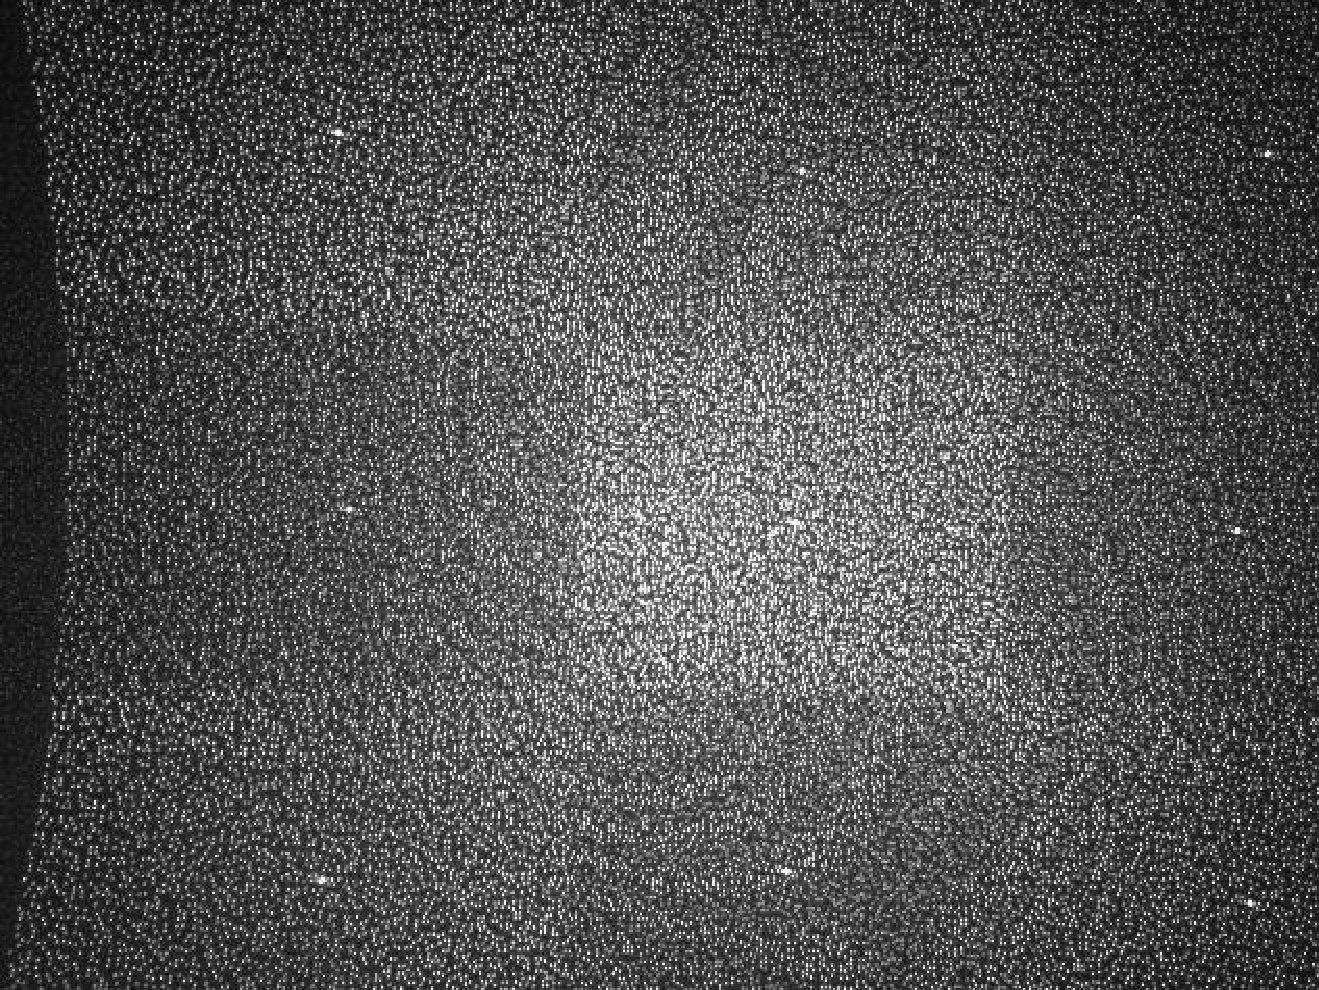
\includegraphics[width=0.8\textwidth]{PrimeSenseInfraredPattern}
%\caption[PrimeSense SL Infrared Pattern.]{
%\begin{varwidth}[t]{\linewidth}
%PrimeSense SL Infrared Pattern. \\%
%Source: \url{http://www.ros.org/wiki/kinect_calibration/technical}
%\end{varwidth}
%}
%\label{PrimeSenseInfraredPattern}
%\end{figure}%
%%
%and an infrared camera inside the scanner is employed to capture images of the target. By comparing part by part to reference patterns, that were captured previously at known depths and stored in the device, the per-pixel depth could be looked up based on the reference pattern that the projected pattern matches best. 
%%\\\\
%After the per-pixel depth data determined from the infrared sensor, the next step would be to correlate to a calibrated RGB data, which will generate a popular unified representation of target's profile: point cloud, a collection of points with \(XYZ\) 3D coordinates and RGB color data. What's more, the surface normals of the target's profile are also stored in every single point of the point cloud data. 
%%
%\\
%\\\textbf{Time of Flight (KinectV2)}\\
%Based on known speed of light, Time-of-Flight (ToF) camera resolves distance by measuring the time cost of a special light signal traveling between the camera and target for every single point. KinectV2 is one of the practical consumer 3D camera that applied the technology of ToF. Using the active modulated infrared source light together with a low-cost CMOS pixel array, KinectV2 realize its an attractive solution that owns compact construction, high accuracy and up to 30 fps frame-rate.\par%
%%
%%
%\begin{figure}[H]
%\centering
%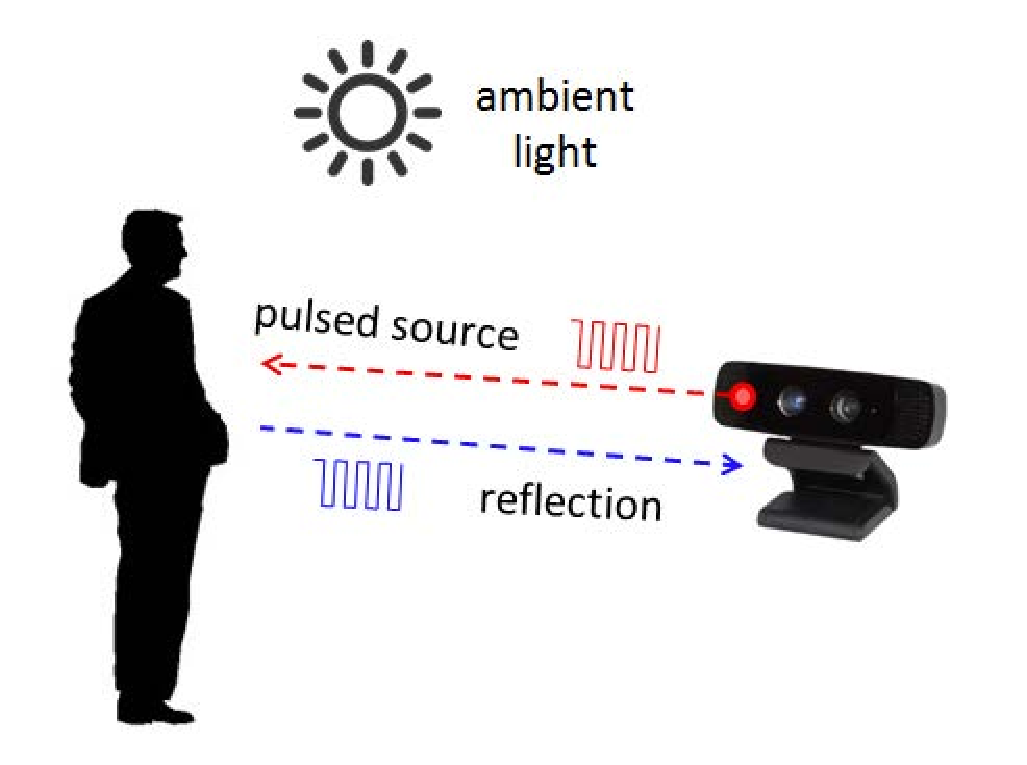
\includegraphics[width=0.7\textwidth]{timeOfFlight}
%\caption{3D time-of-flight camera operation \cite{TimeOfFlight}}
%\label{timeOfFlight}
%\end{figure}%
%%
%\noindent
%The variable that ToF camera measures is the phase shift between the illumination and reflection, which will be translated to distance \cite{TimeOfFlight}. % Texas Instruments Time-of-Flight Camera -An Introduction    Larray Li
%To detect the phase shifts, light source is pulsed or modulated by a continuous wave, typically a sinusoid or square wave.
%As figure \ref{timeOfFlight} shows, the ToF camera illumination is typically from a LED or a solid-state laser operating in the near-infrared range invisible to human eyes. A camera working in the same spectrum captures the reflected light and converts photonic energy to electrical signal, which contains distance (depth) information.
%%\\\\
%The distance measured for every single pixel is saved into a 2D addressable array, which results in a depth map. KinectV2 has a depth map of 512 * 424 unsigned short data collections, which could be finally rendered, together with corresponded RGB stream,  into a tree dimensional space point cloud.
%%%%%%%%%%%%%%%%%%%%%%%%%%%%%%%%%%%%%%%%%%%%%%%%%%%%%%%
%%%%%%%%%%%                                                                         %%%%%%%%%%%%%%%%%%%%
%%%%%%%%%%%  1.3   Structured Light 3D Scanner Calibration       %%%%%%%%%%%%%%%%%%%%
%%%%%%%%%%%                                                                            %%%%%%%%%%%%%
%%%%%%%%%%%%%%%%%%%%%%%%%%%%%%%%%%%%%%%%%%%%%%%%%%%%%%%%
%
%\section{Structured Light 3D Scanner} % (specially with cheap low quality lenses)
%\label{sectionSL3DCalibration} % For referencing the chapter elsewhere, use \ref{sectionSL3DCalibration} 
%
%Structured Light Illumination (SLI) has become the most widely used active vision [12] method for non-contact 3D measurement, applied in the fields of industrial quality control [14, 15], biometrics [16], biomedical topology [13],  archaeologicaldocumentation [9],  and the entertainment industry.  The numerous uses of SLI have lead to an abundance of different methods for the generation of surface topology, although each technique utilizes the basic premise of measuring the specific deformation of a projected light pattern on the surface contours of a target object [17].  The light pattern can take various forms: a spot [12], a single light stripe [17, 18], multiple light stripes[19], a grid[20,21], sine-wave encoded stripes[22], binary encoded stripes, and various other patterns [12].
%
%The way a pattern is utilized to generate 3D information can vary as well, evolving from the classic SLI approach utilizing a single light stripe.  In this classic approach, a single laser stripe is scanned laterally across a surface and a 2D image is captured for each of the points that the stripe intersects.  This causes the 3-D resolution to be directly related to the number if images captured, and drives the inherent costs of processing the data very high.  Improved methods utilizing multiple stripes [19] can capitalize on illuminating the entire surfacein the captured image to gain increased performance,butthese multi-striped patterns introduce ambiguities near discontinuities in the target surface, and can be sensitive to the albedo of the surface.  Using multi-frame pattern techniques in a sequence, each pixel of the image can be encoded to eliminate the reconstruction ambiguities and sensitivity to the albedo surface.  The sequences can consist of color-encoding patterns [23] or binary-encoding patterns [27, 28], but the multi-frame pattern sequence called phase-measuring Profilometry (PMP) [29]is particularly robust and the focus of this Thesis.
%
%PMP encodes the surface points with specific phase values, with increasing depth resolution when using higher frequency patterns.  The downside is that ambiguous reconstruction occurs with higher frequencies, which leads to multiple-frequency PMP techniques [30-32] to resolve the ambiguities with the phase.Using a conventional PMP method, erroneous motion of the target surface causes reconstruction artifacts that are unresolvable; however, a method called Lock and Hold [40, 41]allows thecapture of full 3-D motion with the depth-resolution of a high frequency PMP pattern.   
%
%
%
%
%
%
%
%
%Structured light (SL) technique is the fastest method for 3D reconstruction. By driving the projector / camera pair at very high frame rates, the object's motion then become small over the pattern set. However, at a high frame rate, the process speed of incoming video becomes an issue. Instead of recoding camera frames to memory and then applying off-line processing (like many video-based SL systems chose), Kai \cite{Kai10} made a good research on structured light 3D reconstruction in real-time, which brought in a pinhole-camera model based 3D scanner calibration method. %
%%\\\\%
%To be able to produce 3D point clouds in real-time, Kai proposed a look-up table based solution that is built on the derivation of pinhole camera model 3-by-4 transformation matrix, with a novel dual-frequency pattern. By his method, a 640 by 480 video steam can generate intermediate phase data at 1063.8 frames per second and full 3D coordinate point clouds at 228.3 frames per second, which is a satisfying speed. However, this method, being not able to remove lens distortions, is only one good lead-in 3D camera calibration method.%
%\\\\%
%3D scanner calibration aims to determine the mathematical equation for every single pixel's sight, i.e., to calculate a beam equation. Concretely, with \enquote{depth} (\(Z^{w}\)) value given in RGB-D cameras, the beam equation calculation is to determine the linear translation coefficients from \(Z^{w}\) to \(X^{w}\) and \(Y^{w}\). And how well the calibration is depends on how much distortions are removed in the beam equation.%
%%\\\\%
%Two kinds of distortions need to be taken care of through 3D camera calibration: perspective distortion and lens distortion. Perspective distortion is caused by the position of the camera relative to the subject, or by the position of the subject within the image frame, linear. And lens distortion is caused by optical design of lenses, non-linear. Traditionally and commonly, an ideal pinhole camera model is employed as an simple algorithm in 3D computer vision to describe a mapping from the 3D world coordinates to camera image row and column, by giving a translation method from \(Z^{w}\) to \(X^{w}\)  and \(Y^{w}\)  for every single pixel. It works decently only for ideal pinhole cameras that have no lens, whereas real cameras need extra modifications and supplementations to solve the non-linear radial and tangential lens distortion.%
%%\\\\%
%Totally based on the pinhole camera model (a 3-by-4 matrix), the 3D camera calibration method from Kai's analysis can only take care of the linear perspective distortion, which not able to handle the non-linear radial dominated lens distortion. Details will soon be discussed in in chapter \ref{sens_PinHoleCameraStructuredLight}. %
%
%
%
%
%
%
%
%
%
%
%
%
%
%






%
%
%%%%%%%%%%%%%%%%%%%%%%%%%%%%%%%%%%%%%%%%%%%%%%%%%%%%%%%
%%%%%%%%%%                                                     %%%%%%%%%%%%%%%%%%%%%%%%%%%
%%%%%%%%%%  1.3   Contributions of this thesis             %%%%%%%%%%%%%%%%%%%%%%%%
%%%%%%%%%%                                                     %%%%%%%%%%%%%%%%%%%%%%%%
%%%%%%%%%%%%%%%%%%%%%%%%%%%%%%%%%%%%%%%%%%%%%%%%%%%%%%%
\section{Contributions of this thesis}
%%%%%%	
For RGB-D cameras, RGB steam and Depth steam are two steams that independent but correlated with each other. With respect to every \(X^{w}\)/\(Y^{w}\) correlated single pixel-pair, Depth steam offers the additional voxel world coordinates \(Z^{w}\), while RGB steam offers the additive color property.
%\\\\
As described in section \ref{sectionSL3DCalibration}, even though a pinhole camera model (3-by-4 transformation matrix) could help do 3D scanner calibration, it is only for ideal camera without lens. That is to say, in practical the lens distortions correction is separated from pinhole camera model calibration. Even though same pixel coordinate-pairs (world coordinates and image plane coordinates) could be re-utilized to solve radial dominated lens distortions, as a second step after the determination of a 3-by-4 pinhole camera model, the calculation of the separated step brings a second-time translation cost for every single pixel of every frame. This is not a good way to do real-time reconstruction. %
\\\\%
In order to remove the radial dominated lens distortions, two 3D camera calibration methods, got inspired from Kai's method, are proposed and discussed. The first method inherits the advantages given by the pinhole camera model, which can offer the relationship between \(Z^{w}\) and \(X^{w}\)/\(Y^{w}\) for every single pixel as long as its field of view is pre-calculated. This method is only discussed theoretically, because the second method is simpler, more accurate, and is finally applied into practical calibration.%
%\\\\%
Thoroughly abandoned the pinhole camera model, the second method directly determines the beam equation for every single pixel by collecting distortions-removed \(X^{w}\)/\(Y^{w}\) and accurate \(Z^{w}\) values. \(X^{w}\)/\(Y^{w}\) values are calibrated by high order, concretely \(4th\) order, polynomial surface mapping. And the accurate \(Z^{w}\) values are imported from external \(Z^{w}\)-aixs tracking module. In short, this is totally a data-based calibration method.%
%
\begin{figure}[H]
\centering
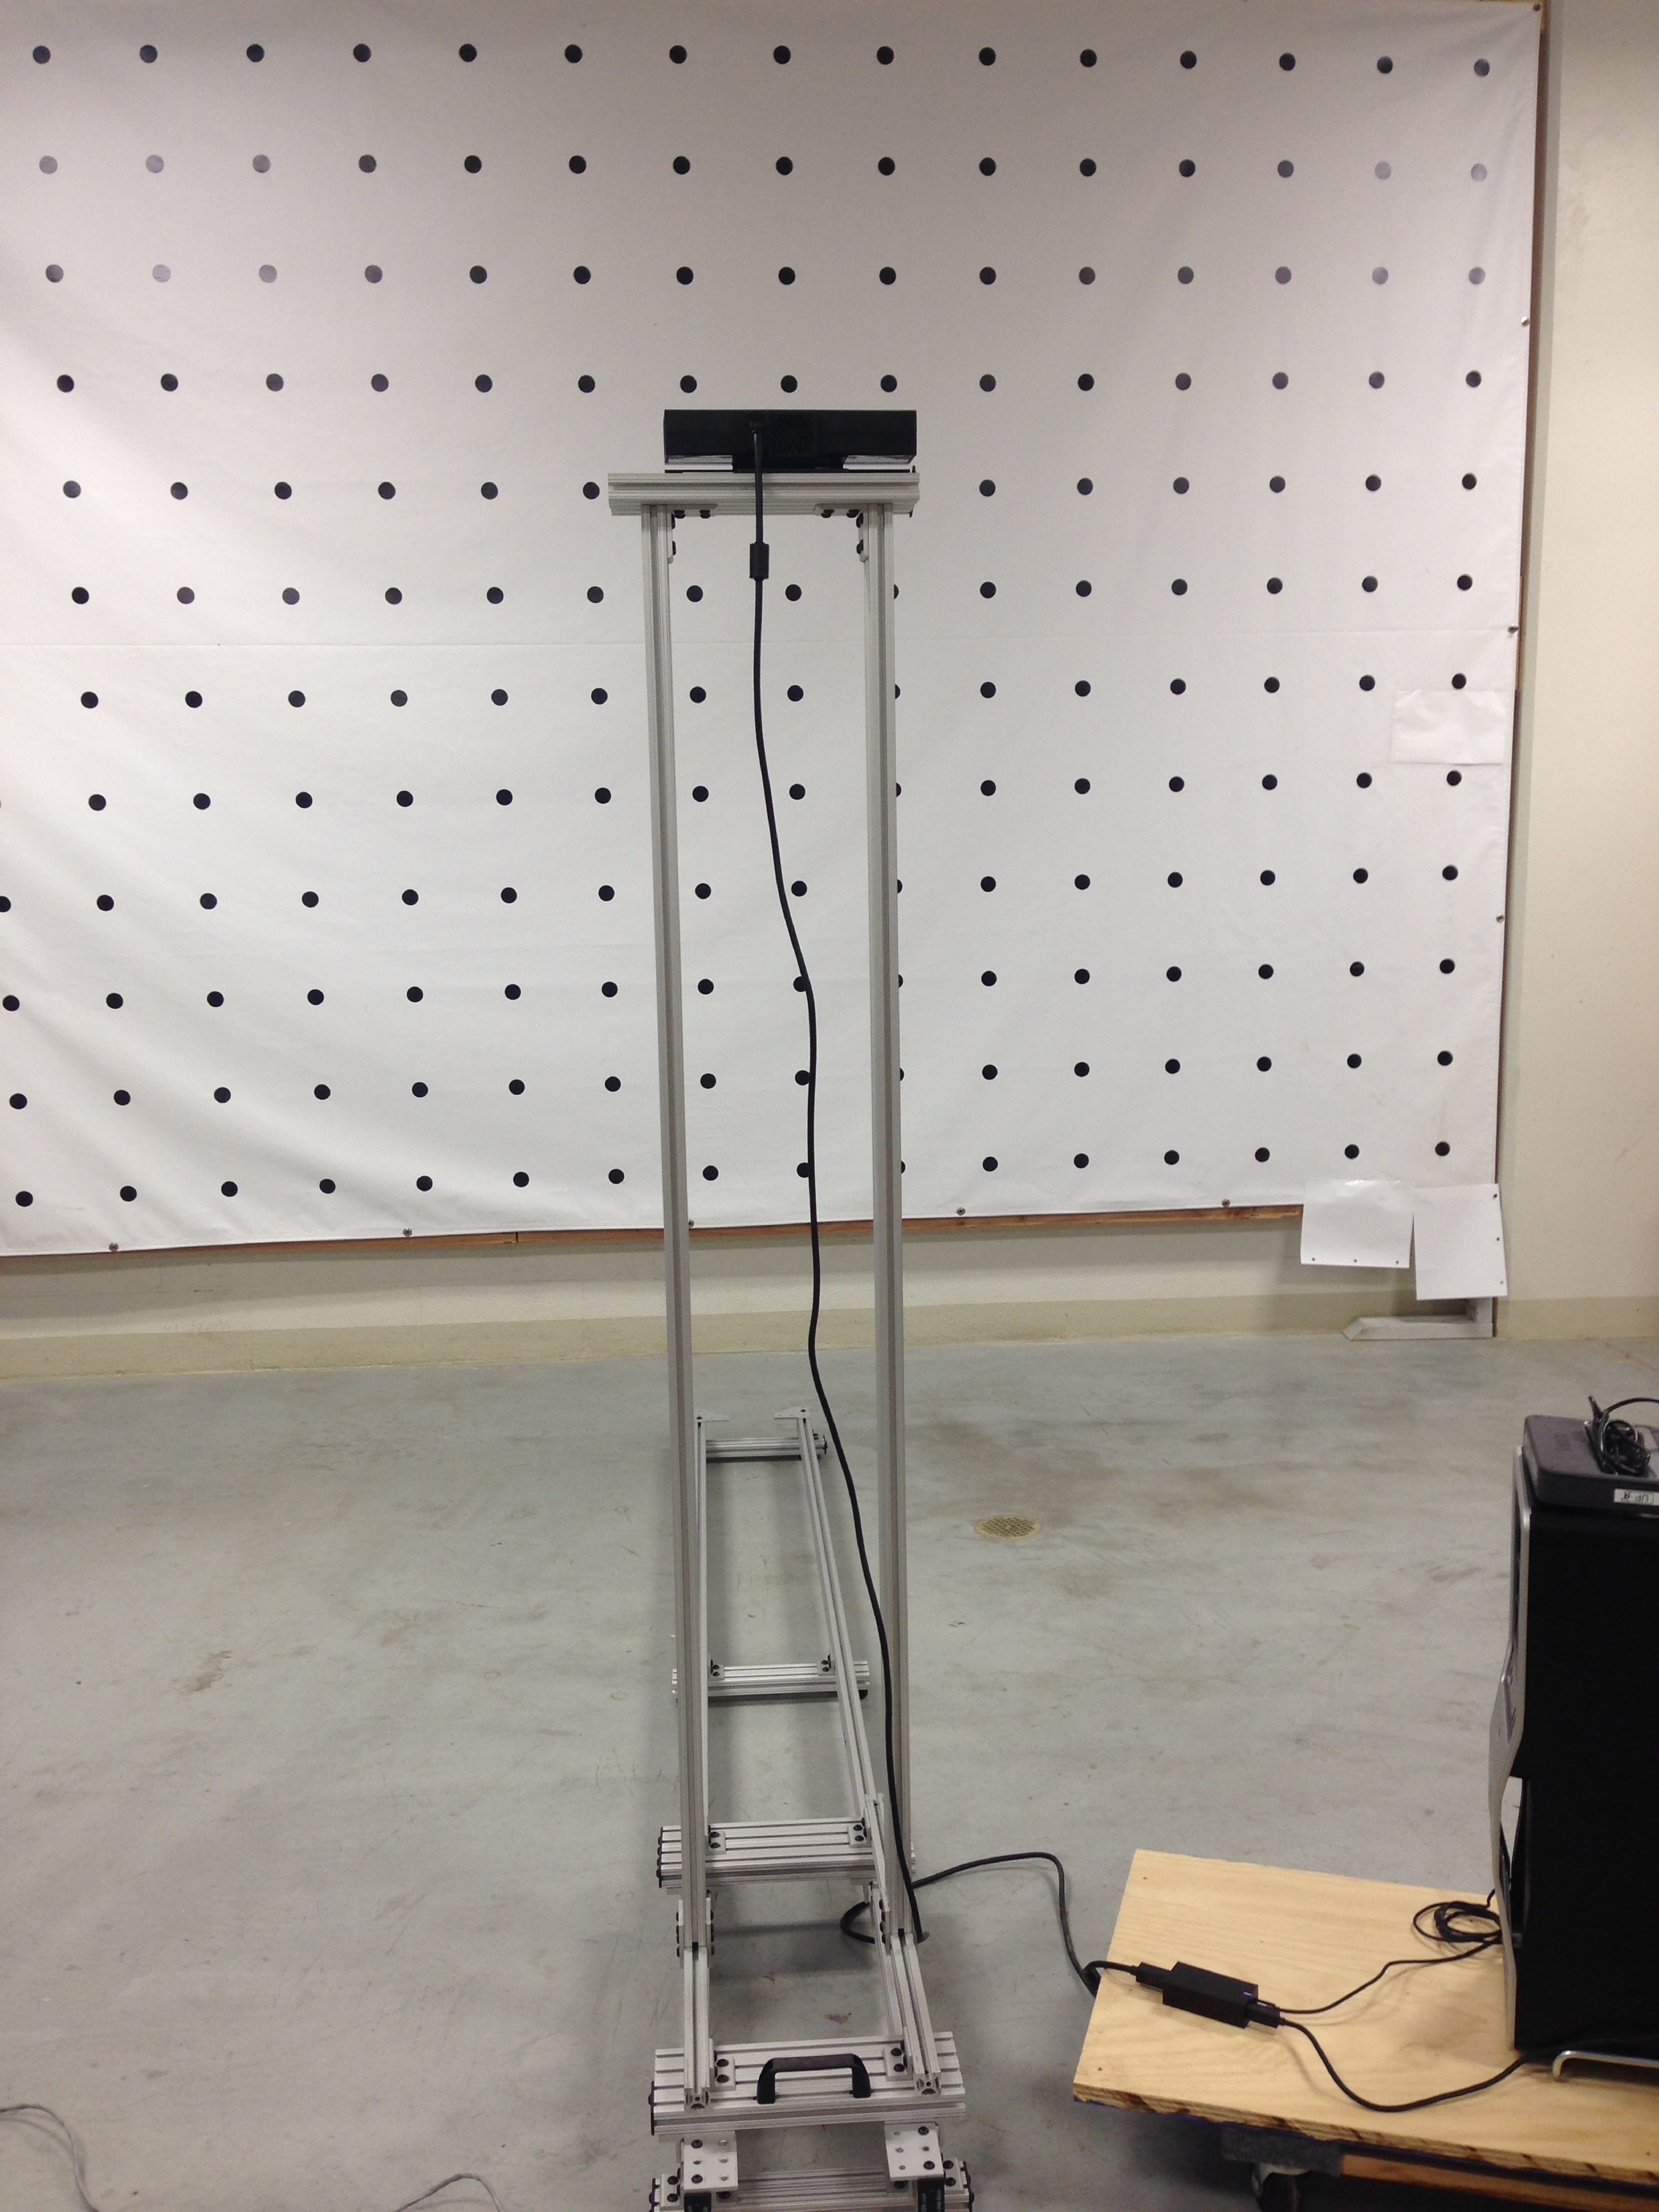
\includegraphics[width=0.5\textwidth]{trackingModuleOnKinectV2CalibrationSystem}
\caption{KinectV2 Calibration System}
\label{trackingModuleOnKinectV2CalibrationSystem}
\end{figure}%
%
\noindent
To collect enough data along \(Z^{w}\)-aixs, a rail is used in the calibration system. As shown in figure \ref{trackingModuleOnKinectV2CalibrationSystem}, the rail is perpendicular to the uniform round dot pattern as \(Z^{w}\) axis. A RGB-D camera KinectV2 is mounted on the top of the slider, while a BLE OF tracking module is specially designed and mounted at the bottom of the slider, observing the rail and supporting accurate \(Z^{w}\) values. With this calibration system that helps collect data easily, a distortion-removed XYZ-D Look-Up Table (LUT) will be generated for real-time 3D reconstruction.%
%%%%%%%%%%%%%%%%%
%%%%%%%%%%%%%%%%%
%%%%%%%%%%%%%%%%%
%%%%%%%%%%%%%%%%%

\section{Summation}

 RGB-D cameras' calibration cannot be easily handled by a pinhole camera model. First of all, as mentioned in section \ref{sectionSL3DCalibration} and detailed in section \ref{sectionPinholeCamera}, a pinhole camera model is not able to handle the non-linear radial dominated lens distortion. What's worse, the depth resolution deteriorates notably with depth in practical \cite{Krystof12}, so such so that the \(depth\) values are not able to guarantee an accurate  \(Z^{w}\).
%
 \begin{figure}[H]
%\centering
\subfloat[Front View][Front View]{
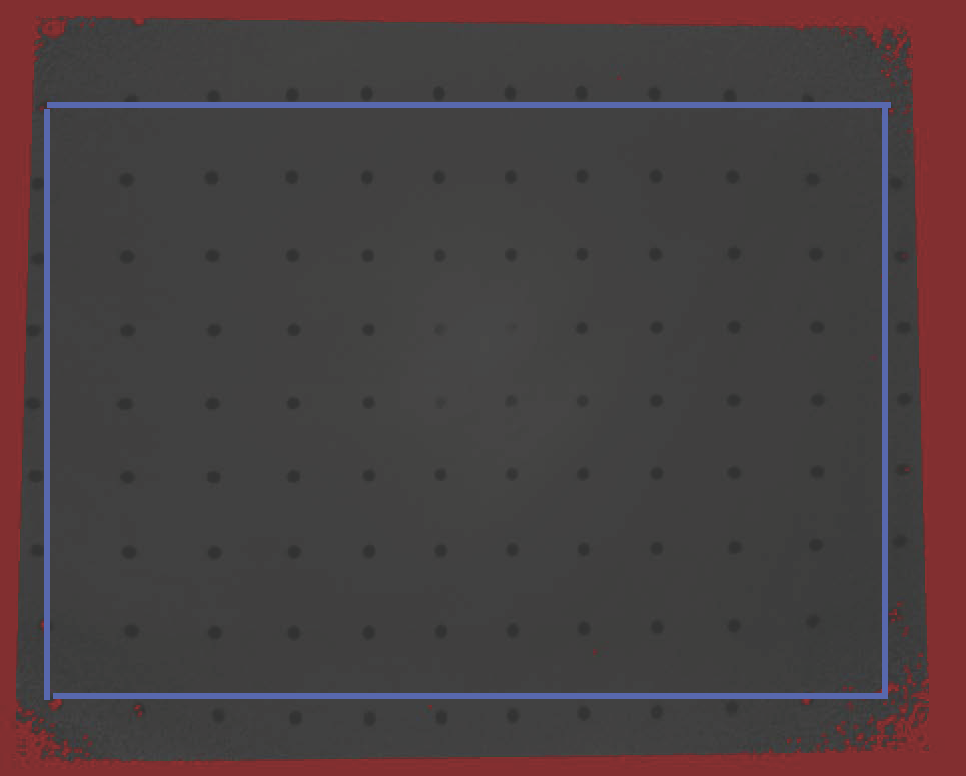
\includegraphics[height=0.42\textwidth]{NIR_by_Depth_front}
\label{NIR_by_Depth_front}}
\subfloat[Left View][Left View]{
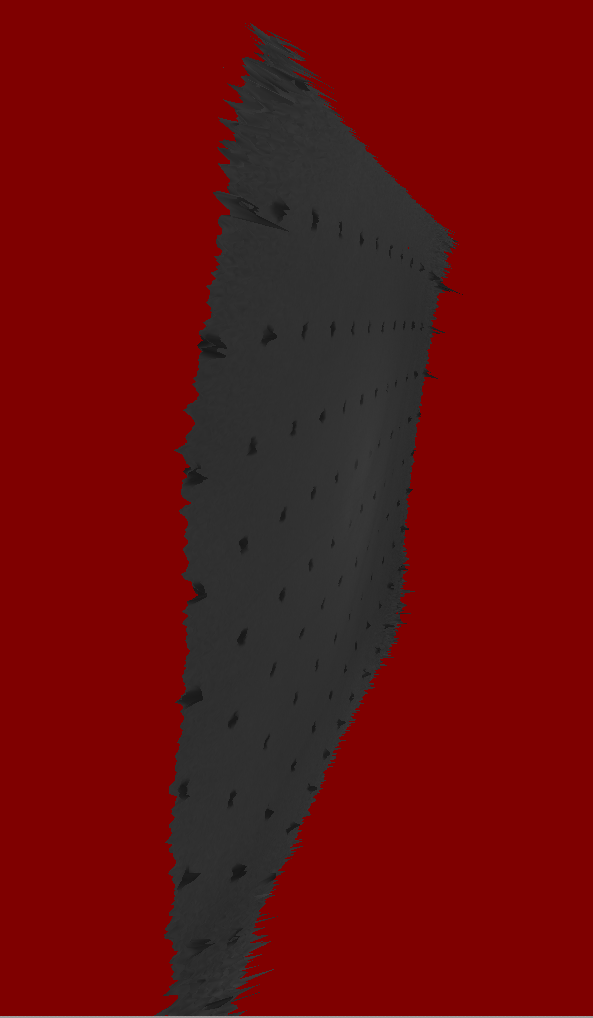
\includegraphics[height=0.42\textwidth , width = 0.4\textwidth]{NIR_by_Depth_LeftSide}
\label{NIR_by_Depth_LeftSide}}
%\qquad
\caption{Raw NearIR 3D Reconstruction based on Pinhole Camera Model}
\label{NearIR}
\end{figure}%
%
\noindent
Noises among depth data vary randomly, camera by camera and pixel by pixel; which means a rough point-cloud plane full of bumps and hollows will be reconstructed even though the camera is observing a wall. As shown in figure \ref{NIR_by_Depth_LeftSide}, the blue straight line should be the left side of the 3D reconstruction, whereas most pixels on the left side border are apparently not sitting on a straight line.%
%
Got inspired and extended from Kai's 3D reconstruction research, a data-based XYZ-D LUT calibration method is proposed and applied into practical application, with the help of a specially designed BLE OF tracking model supporting external accurate \(Z^{w}\) values. In applying this method, not only lens distortion, but also depth distortion can be removed from the 3D coordinates for reconstruction.%
\\\\%
In Chapter 2, a pinhole camera model based calibration method is discussed in detail, from which two extended calibration methods are proposed and discussed. The second proposed method is well explained in Chapter 3. \(X^{w}\) and \(Y^{w}\) are mapped separately through a fourth order surface fitting translation from image plane row and column to directly solve the lens distortion problem. Then, \(Z^{w}\) values are totally supported from external BLE optical-flow sensor, which accurately tracks camera movements along Z-axis. Chapter 4 will introduce the whole calibration system, with the individually designed BLE OF tracking module. Finally, a data-based XYZWRGB-D look-up table will be generated for real-time reconstruction.




































